%%%%%%%%%%%%%%%%%%%%%%%%%%%%%%%%%%%%%%%%%%%%%%%%%%%%%%%%%%%%%%%%%%%%%%%%%%%%%%%%%%%%%%%%%
%%                                                                                     %%
%%                This file is part of the CAPH Compiler distribution                  %%
%%                            http:%/caph.univ-bpclermont.fr                           %%
%%                                                                                     %%
%%                                  Jocelyn SEROT                                      %%
%%                         Jocelyn.Serot@univ-bpclermont.fr                            %%
%%                                                                                     %%
%%         Copyright 2011-2018 Jocelyn SEROT.  All rights reserved.                    %%
%%  This file is distributed under the terms of the GNU Library General Public License %%
%%      with the special exception on linking described in file ..%LICENSE.            %%
%%                                                                                     %%
%%%%%%%%%%%%%%%%%%%%%%%%%%%%%%%%%%%%%%%%%%%%%%%%%%%%%%%%%%%%%%%%%%%%%%%%%%%%%%%%%%%%%%%%%

\chapter{Introduction}
\label{chap:intro}

This document describes the \caph programming language.  \caph\footnote{\caph stands for \emph{Caph
    just Ain't Plain HDL}. \emph{Caph} is also the name of the second bright star in the
  constellation of Cassiopeia.} is a domain-specific, high-level language for programming FPGAs.
\caph is based upon the \emph{dataflow process network} model of computation~\cite{DPN} and
produces implementations relying on a pure \emph{data-driven} execution model.  The \caph compiler
is able to generate synthetizable VHDL code from high-level descriptions of programs as networks of
interconnected dataflow actors.

\medskip This report is structured as follows: the remainder of this chapter provides motivation and
general background; Chapter~\ref{chap:overview} is an overview of the \caph language design,
including informal descriptions of the expression, network and actor sub-languages. The full
concrete syntax is given in chapter~\ref{chap:syntax} and the abstract syntax of the core language
in chapter~\ref{chap:abssyn}. Chapter~\ref{chap:typing} gives the formal typing rules for \caph
programs. Chapter~\ref{chap:static} gives the formal static semantics,
\emph{i.e.} the interpretation of \caph programs as \emph{data-flow graphs}.
Chapter~\ref{chap:dynamic-semantics} gives the formal dynamic semantics, which provides a way to
\emph{simulate} \caph programs.  Chapter~\ref{chap:interm-repr} describes
  the intermediate representation of \caph programs used as an input for the back-end code
  generators. Chapter~\ref{cha:using-caph-compiler} describes, pragmatically, how to use the
compiler in order to obtain graphical representations of programs, simulate them or invoke the
SystemC or VHDL backend in order to generate code. Chapter~\ref{cha:stdlib} gives the contents of
some ``standard libraries''. Chapter~\ref{cha:foreign-funct-interf} describes
the mechanism by which existing C or VHDL functions can be used by \caph
programs. Chapter~\ref{cha:compiler-options} is a summary of compiler options.
 Chapter~\ref{cha:variants-impl} is a short, technical, overview of how \emph{variant
  types} (described in chapter~\ref{chap:overview}) are implemented in SystemC and VHDL. 

\clearpage

\section{Motivation, goals and principles}

The design of the \caph language was guided by the following motivations and general principles:

\medskip \textbf{Specificity}. Although most of its underlying concepts are very general -- and
could indeed be applied to a large variety of programming languages targetting either software or
hardware --, the \caph language has been primarily designed to program FPGAs. This deliberate
orientation allowed us to make clear and argumented choices regarding the set of supported
features.
Other languages relying on the same model of computation (MoC) -- such as \textsc{cal}~\cite{CAL}
for example -- are less specific, targeting both software and hardware implementations, and
sometimes offer a richer set of features. But this richness comes at the price of ambiguity
since it's frequent that not all features are supported in hardware implementations. Moreover, the
set of supported features is not always clearly documented and must often be defined by tedious,
repeated experiments. Our approach is more pragmatic, if less ambitious: if it can be described, it
can be implemented.

\medskip
\textbf{Formal basis}. We strongly adhere to the idea that any decent programming language should be
based upon formal semantics, describing in a complete and unambiguous manner the meaning of
programs. The essentially \emph{functional} orientation of \caph greatly eases the
writing of such semantics. It also makes it possible to describe formally, and
in a platform-independant way, the transformation process by which the high level language source
code is turned into low-level VHDL code, a highly desirable property in our case, since it allows 
reasoning about this process (for certification and optimization purposes for example). Another
advantage is the ability to derive (in a systematic way) a reference interpreter for the
language. Such a reference interpreter can then be used latter to assess the correctness of the
results produced by generated low-level code.

\medskip
\textbf{Minimum distance} between the programming model and the execution model. This is the key
idea for being able to produce efficient low-level harware solutions from high-level descriptions
while keeping adherence to the second principle. Abstraction and efficiency being generaly
perceived as contradictory requirements, this principle is often interpreted as : keep the the
abstraction low at source level. Fortunately, this is not the case with the dataflow programming
and execution models \caph is relying on. A large part of this is due to the natural affinity
between the dataflow MoC and the concepts used in purely functional programming languages (absence
of side-effects, polymorphic type systems, higher-order constructs).

\medskip
Beside these general principals, \caph was also developped with a set of more technical / pragmatical
goals in mind :

\medskip
\textbf{Strict separation of concerns} between computation and communication. This is reflected by
the structure of the language, which embeds an
\emph{expression language} (for describing computations) within
a \emph{declaration language} (for describing the global structure of the program) on the one hand,
and provides two separate sub-languages for describing the behavior of actors and the communication
network by which these actors interact, on the other hand.

\medskip
\textbf{Composability, modularity}. This refers to the ability to build large, complex applications
from smaller, simpler ones. This is naturally supported by the dataflow model of computation (no
shared variables and hence no hidden dependencies) and the purely functional coordination language
(referential transparency).

\medskip
\textbf{Reuse}. Within the language, this is supported by \emph{higher-order} constructs. At the
actor level, higher-order actors can be used to encapsulate recurrent patterns of
\emph{computations}. At the network level, higher-order functions can be used to encapsulate recurrent patterns of
\emph{communication}. \caph also offers the ability to import legacy existing code (in VHDL for
synthesis, in C/SystemC for simulation).

\medskip
\textbf{Arbitrary data structuring}. By this we mean the ability to encode values -- and, jointly,
to describe actors operating on these values -- having an arbitrarily complex data structure.
In particular, the language should support the description of operations on 
non-regular and/or or variable-sized data structures (lists or trees, as opposed to fixed-sized
arrays, for instance). In other words, the target applications should not be limited to regular
signal or image processing. In \caph, this is provided by separating the tokens exchanged by actors
into two classes : \emph{data tokens} (carrying actual values) and \emph{control tokens} (acting as
structuring delimiters). 

\section{Language principles}
\label{sec:language-principles}

\caph is based upon the \emph{dataflow process network} model of computation~\cite{DPN}.
Applications are described networks of computational units, called \emph{actors}, exchanging
\emph{streams} of tokens through FIFO channels.
Interaction between actors is strictly limited to token exchange
through channels, so that the behavior of each actor can be completely described in terms of actions
performed on its inputs to produce outputs (no side effect, strictly local control).

We will illustrate this model with a very simple example, involving four basic actors. These actors
are depicted Fig.~\ref{fig:fouractors}. Actor \texttt{INC} (resp. \texttt{DEC}) adds
(resp. substracts) 1 to each element of its input stream. Actor \texttt{MUL} performs point-wise
multiplication of two streams. Actor \texttt{DUP} duplicates its input stream\footnote{In
  Fig.~\ref{fig:fouractors}, streams are denoted (ordered) from right to left; for example, the
  actor \texttt{ADD} first processes the token \texttt{1}, then the token \texttt{2}, \emph{etc.}
  Since streams are potentially infinite, their end is denoted ``\texttt{...}''. However, when describing
  actors \emph{textually}, streams will be denoted from left to right; for example:
  \texttt{ADD:1,2,... = 2,3,...}}. Now, if we connect
these four actors to build the network depicted in Fig~\ref{fig:networkfour}, this network computes
$f(x)=(x+1)\times(x-1)$ for each element $x$ of its input stream. I.e. if the input stream \emph{i}
is \texttt{1,2,3,...}, then the output stream \emph{o} will be \texttt{0,3,8,...}

\begin{figure}[h]
  \centering
  \includegraphics[width=1.0\textwidth]{figs/fouractors}
  \caption{Four basic actors}
  \label{fig:fouractors}
\end{figure}

\begin{figure}[h]
  \centering
  \includegraphics[width=0.75\textwidth]{figs/networkfour}
  \caption{A dataflow process network}
  \label{fig:networkfour}
\end{figure}

\medskip
Such a model of computation is indeed very general and can be interpreted in different ways, 
depending in particular in 
\begin{itemize}
\item the kind of behavior that can be assigned to actors (purely functional, stateful, firing
  semantics, \ldots),
\item the exact nature of channels (single place buffer / FIFO, bounded / unbounded, \ldots),
\item how networks are described.
\end{itemize}

In \caph
\begin{itemize}
\item the behavior of actors is specified using a set of \emph{transition rules} using \emph{pattern
    matching} and
  actors are stateful,
\item channels are bounded FIFOs,
\item networks are described in a \emph{implicit} manner, using a set of \emph{functional
    equations}.
\end{itemize}
These aspects are detailed in the next section.

\section{Language Structure}
\label{sec:language-structure}

In common with other coordination language approaches such as 
Hume~\cite{Hume}, \caph takes a layered approach (see Fig.~\ref{fig:languagestruct}).

\begin{figure}[h]
  \centering
  \includegraphics[width=0.75\textwidth]{figs/languagestruct}
  \caption{Caph language structure}
  \label{fig:languagestruct}
\end{figure}

The outermost (\emph{declaration}) layer declares types, global values (constant and functions), I/O streams, actors and
network-level objects (wires and wiring functions).

The innermost (\emph{expression}) layer is a small, purely functional language used for describing
values and computations. This language is used both for defining the values assigned to global constants and
functions and the values computed by actors.

At an intermediate level, two sub-languages can be distinguished : an \emph{actor} sub-language,
used for describing the interface and the behavior of actors, and a \emph{network} sub-language,
used for describing the structure of the dataflow process network. 
Both languages are functionnaly-based, 

\subsection{The network language}
\label{sec:network-lang}

The \caph\ {\it network language} is used for describing the structure of the dataflow process
network describing the program. It is purely functional, polymorphic and supports higher-order
functions. It is largely inspired from previous work on the \fgn system ~\cite{FGN}.

The basic unit of coordination is the {\it box}. A \emph{box} is an instance of an actor, viewed
abstractly, \emph{i.e.} only retaining its interface (parameters and input/output ports). 
The network language is responsible for describing the \emph{wiring} of these boxes to form the
dataflow process network corresponding to the program to be implemented (including the connections to the
external devices).  

The basic concept is that the network of actors is actually a dataflow graph (DFG) and that a DFG can
be described by means of purely functional expressions~\cite{SerotQZ95}.

Consider for example, the minimal network depicted in Fig.~\ref{fig:smallnet1}, in which
\texttt{inc} is an actor with one input and one output, \texttt{i} an input stream and \texttt{o}
an output stream\footnote{This figure has been produced with the \caph graph visualizer. Actors are
  drawn as rectangular boxes and I/O streams as triangles.}. It can be described with the following
\caph declaration :

\begin{alltt}
net o = inc i;
\end{alltt}

\begin{figure}[h]
  \centering
  \includegraphics[height=1.5cm]{figs/smallnet1}
  \caption{A minimal actor network}
  \label{fig:smallnet1}
\end{figure}

This declaration
\begin{enumerate}
\item instanciates the \emph{inc} actor, i.e. creates a box in the network,
\item connects the network stream input \texttt{i} to the input of this box,
\item connects the network stream output \texttt{o} to the output of the \texttt{inc} box.
\end{enumerate}

\medskip Usage of \texttt{net} declarations is of course not limited to binding network
outputs. They are generally used to bind the output(s) of a box, in order to reuse it (them) in subsequent
declarations, thus ``wiring'' the network. Such values are therefore called ``wires'' in the network language. A
minimal example for this is given in Fig.~\ref{fig:smallnet2}, where two instances of the
\texttt{inc} actor are wired together.

Note that the same network could have been described without
naming the intermediate wire, by writing just : \texttt{net o = inc (inc i);}

\begin{figure}[h]
  \centering
  \begin{tabular}[t]{cc}
    \begin{minipage}[c]{0.5\linewidth}
      \begin{lstlisting}
        net x = inc i;
        net o = inc x;
      \end{lstlisting}
    \end{minipage}
\adjustbox{valign=c}{\includegraphics[width=0.5\linewidth]{figs/smallnet2}}
  %\includegraphics[width=0.5\linewidth]{figs/smallnet2}
  \end{tabular}
  \caption{A small actor network}
  \label{fig:smallnet2}
\end{figure}

\medskip The network depicted in Fig.~\ref{fig:networkfour} can be described with the following
\caph declarations\footnote{Provided that the \texttt{dup}, \texttt{inc}, \texttt{dec} and \texttt{mul} actors
have been previously declared with the right interface and that \texttt{i} and \texttt{o} designate
the input and output of the network.}, showing in particular how multiple outputs of an actor can be
bound, using a tuple value :

\begin{lstlisting}
net (i1,i2) = dup i;
net o = mul (inc i1, dec i2);
\end{lstlisting}

\medskip
Compared to other textual or graphical network languages, this notation offers a
significantly higher level of abstraction. In particular it saves the programmer from having to
explicitly describe the wiring of channels between actors, a tedious and error-prone task. 
Moreover, ill-formed networks and inconsistent use of actors can be readily detected using a
classical Hindley-Milner polymorphic type-checking phase. 

Another advantage of ``encoding'' data-flow networks in a functional language
is the ability to define reusable, polymorphic \emph{graph patterns} in the form of higher-order
functions, which offers an easy and safe compositional approach for building larger applications from smaller ones.

For example, the network of Fig~\ref{fig:networkfour} could also have been described with the
following declarations, in which the \texttt{diamond} function \emph{encapsulates} the diamond-shaped graph
pattern examplified here :

\begin{lstlisting}[frame=single]
net diamond (left,top,bottom,right) x = 
  let (x1,x2) = left x in
  right (top x1, bottom x2);

net o = diamond (dup,inc,dec,mul) i;
\end{lstlisting}

The \texttt{diamond} function is called a \emph{wiring function} in the \caph network language. From a 
functional perspective, this is a \emph{higher-order} function, i.e. a function taking other
function(s) as argument(s). Once defined, such a function can be reused to freely instanciate graph
patterns. For example, the network depicted in Fig~\ref{fig:diamonds}, in which the ``diamond''
pattern is instanciated at two different hierarchical levels, can be simply described with the
following declaration~:

\begin{lstlisting}
net o = diamond (dup, inc, diamond (dup,inc,dec,mul), mul) i;
\end{lstlisting}

\begin{figure}[h]
\begin{center}
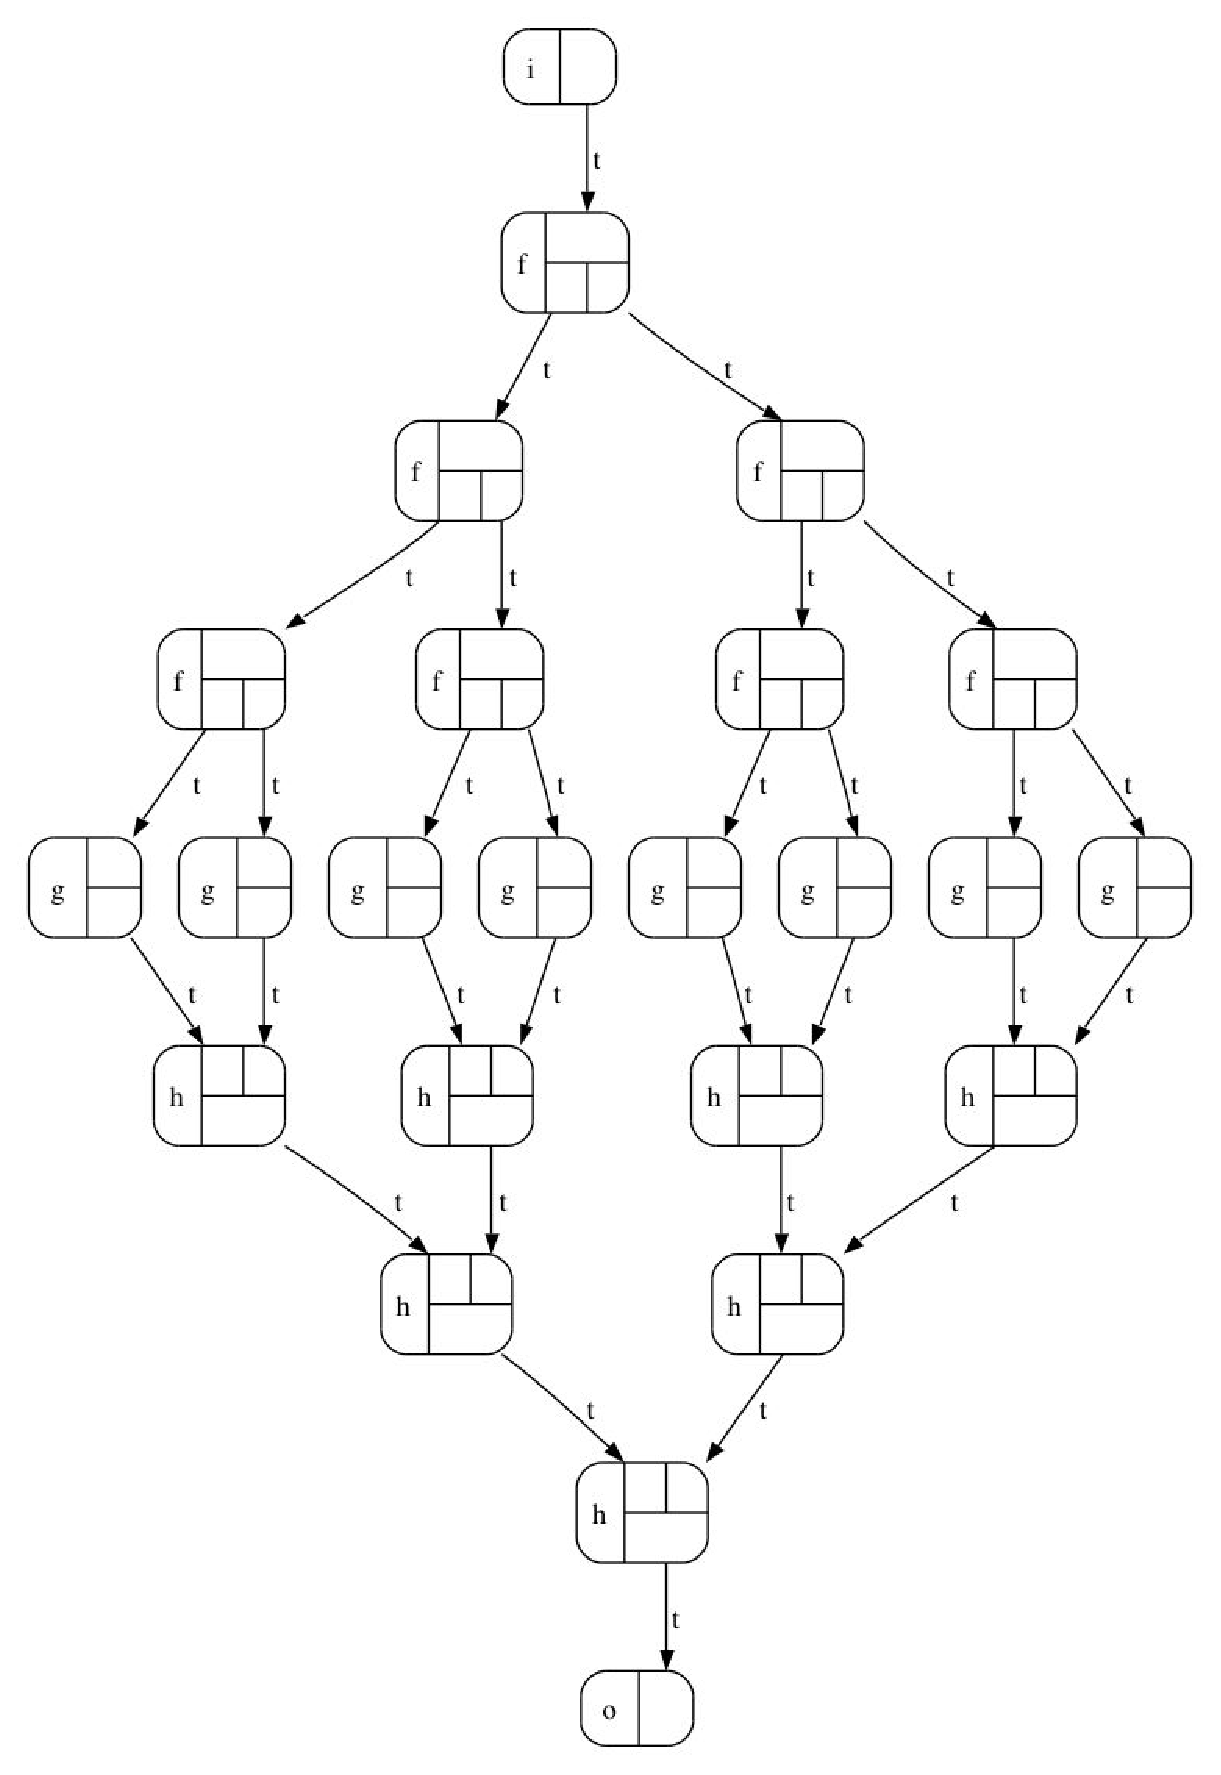
\includegraphics[width=0.85\textwidth]{figs/diamonds}
\caption{A hierachical network}
\label{fig:diamonds}
\end{center}
\end{figure}

\subsection{The actor Language}
\label{sec:actor-lang}

The \caph\ {\it actor language} is used to describe the behavior of individual dataflow actors. 
This is done using a set of \emph{transition rules}, fired according to a generalized
pattern-matching mechanism. The actions performed by each rule are described using a purely functional, primitive recursive
language with a strict semantics.

A complete description of the actor language will be given in the next chapter. In this section, we
will just introduce it using a simple example. Let us consider the actor \texttt{merge} described in
Fig.~\ref{fig:mergeactor}. This actor takes two streams of tokens as inputs and produces one stream
of tokens, taking input alternately from the first and second output.  Its behavior description in
\caph is given on the left. It has two inputs and one output, all of type \texttt{int}. It also
uses a local variable, \texttt{s}, of type \texttt{bool}.
Its behavior is specified using a set of rules defined under the \texttt{rules} keyword.
Each rule consists of a set of \emph{patterns} refering to inputs or local variables and a
corresponding set of \emph{expressions}, refering to outputs or local variables.
The first (resp. second) rule
says : If \texttt{s} is \texttt{'false'} (resp. \texttt{'true'}) and a value \texttt{v} is available
on input \texttt{i1} (resp. \texttt{i2}) then read\footnote{Pop the connected channel.}
this value, write it to output \texttt{o} and set \texttt{s} to \texttt{'true'}
(resp. \texttt{'false'}).

Fig.~\ref{fig:fouractorsdesc} gives the description in \caph of the four actors introduced in
Fig.~\ref{fig:fouractors}. 

\begin{figure}[h]
  \centering
  \includegraphics[width=\linewidth]{figs/mergeactor}
  \caption{An example of actor description in \caph}
  \label{fig:mergeactor}
\end{figure}

\begin{figure}[h]
  \centering
  \begin{tabular}[c]{cc}
    \begin{minipage}[c]{0.45\linewidth}
      \begin{lstlisting}
        actor inc 
          in (i: int)
         out (o: int)
        rules
          i:x -> o:x+1;
      \end{lstlisting}
    \end{minipage} &
    \begin{minipage}[c]{0.45\linewidth}
      \begin{lstlisting}
        actor dec 
          in (i: int)
         out (o: int)
        rules
          i:x -> o:x-1;
      \end{lstlisting}
    \end{minipage} \\
    \begin{minipage}[c]{0.45\linewidth}
      \begin{lstlisting}
        actor mul 
          in (i1: int, i2:int)
         out (o: int)
        rules
          (i1:x, i2:y) -> o:x+y;
      \end{lstlisting}
    \end{minipage} &
    \begin{minipage}[c]{0.45\linewidth}
      \begin{lstlisting}
        actor dup 
          in (i: int)
         out (o1: int, o2: int)
        rules
          i:x -> (o1:x, o2:x);
      \end{lstlisting}
    \end{minipage}
  \end{tabular}
  \caption{\caph description of the four actors introduced in Fig.~\label{fig:fouractorsdesc}}
\end{figure}



\section{Tools and design flow}

The current tool chain supporting the \caph language is sket\-ched on Fig.~\ref{fig:toolset}. It
comprises a graph visualizer, a reference interpreter and compiler producing both SystemC
and synthetizable VHDL code.

\begin{figure}[t]
  \centering
  \includegraphics[width=0.5\textwidth]{figs/toolset}
  \caption{}
  \label{fig:toolset}
\end{figure}

The \textbf{graph visualizer} produces representations of the actor network in the \texttt{.dot}
format~\cite{North1994}
for visualisation with the \textsc{graphviz} suite of tools~\cite{graphivz}.

The \textbf{reference interpreter} implements the dynamic semantics defined in
Sec.~\ref{chap:dynamic-semantics}. 
 Its role is to provide
reference results to check the correctness of the generated SystemC and VHDL code. It can also be
used to test and debug programs, during the first steps of application development (in this case,
input/output streams are read from/written to files). Several 
tracing and monitoring facilities are provided. For example, it is possible to compute statistics on
channel occupation or on rule activation.

The \textbf{compiler} is the core of the system. It relies on an \emph{elaboration phase}, turning
the AST into a target-independant intermediate representation (described in
chapter~\ref{chap:interm-repr}), and a set of dedicated back-ends.

Two back-ends are currently provided : the first produces cycle-accurate SystemC code for simulation
and profiling, the second VHDL code for hardware synthesis. Execution of the SystemC code provides
informations which are used to refine the VHDL implementation (for example : the actual size of the
FIFOs used to implement channels).

\medskip
The graph visualizer, the reference interpreter and the compiler all operate on an abstract syntax
tree (AST) produced by the \textbf{front-end} after parsing and type-checking.

%%% Local Variables: 
%%% mode: latex
%%% TeX-master: "caph"
%%% End: 
